% =====================================================================
% ELMED219: Grafteori og nettverksvitenskap (N01-N10)
% Beamer-presentasjon i widescreen (16:9)
% =====================================================================
\documentclass[aspectratio=169, 11pt]{beamer}

% =====================================================================
% PAKKER
% =====================================================================
\usepackage[utf8]{inputenc}
\usepackage[T1]{fontenc}
\usepackage[norsk]{babel}
\usepackage{graphicx}
\usepackage{tikz}
\usepackage{booktabs}
\usepackage{amsmath}
\usepackage{fontawesome5}

% =====================================================================
% TEMA OG FARGER
% =====================================================================
\usetheme{Madrid}
\usecolortheme{default}

\definecolor{uibblue}{RGB}{0, 61, 115}
\definecolor{uibred}{RGB}{175, 28, 44}
\definecolor{lightgray}{RGB}{245, 245, 245}

\setbeamercolor{palette primary}{bg=uibblue, fg=white}
\setbeamercolor{palette secondary}{bg=uibblue!80, fg=white}
\setbeamercolor{palette tertiary}{bg=uibblue!60, fg=white}
\setbeamercolor{structure}{fg=uibblue}
\setbeamercolor{title}{fg=uibblue}
\setbeamercolor{frametitle}{fg=uibblue, bg=lightgray}
\setbeamercolor{block title}{bg=uibblue, fg=white}
\setbeamercolor{block body}{bg=lightgray}

\setbeamertemplate{navigation symbols}{}
\setbeamertemplate{footline}{
    \hfill\insertframenumber/\inserttotalframenumber\hspace{2mm}\vspace{2mm}
}

% =====================================================================
% TITTELINFO
% =====================================================================
\title[N: Grafteori]{Grafteori og Nettverksvitenskap}
\subtitle{Momentliste N01--N10}
\author{ELMED219 / BMED365}
\institute{Universitetet i Bergen}
\date{Våren 2026}

% =====================================================================
% DOKUMENT
% =====================================================================
\begin{document}

% ---------------------------------------------------------------------
\begin{frame}
    \titlepage
\end{frame}

% ---------------------------------------------------------------------
\begin{frame}{Oversikt}
    \tableofcontents
\end{frame}

% =====================================================================
\section{Grunnleggende grafteori}
% =====================================================================

% ---------------------------------------------------------------------
% N01
% ---------------------------------------------------------------------
\begin{frame}{N01: Hva er en graf? (Noder og kanter)}
    
    \begin{columns}
        \begin{column}{0.45\textwidth}
            \begin{block}{Definisjon}
                En \textbf{graf} $G = (V, E)$ består av:
                \begin{itemize}
                    \item $V$: mengde av \textbf{noder} (vertices)
                    \item $E$: mengde av \textbf{kanter} (edges)
                \end{itemize}
            \end{block}
            
            \vspace{3mm}
            
            \textbf{Medisinsk eksempel:}
            \begin{itemize}
                \item Noder = Pasienter
                \item Kanter = Likhet mellom pasienter
            \end{itemize}
        \end{column}
        
        \begin{column}{0.5\textwidth}
            \begin{center}
                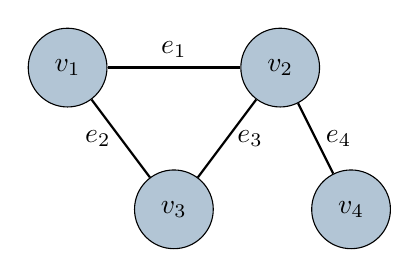
\begin{tikzpicture}[scale=0.9]
                    \node[draw, circle, fill=uibblue!30, minimum size=1cm] (A) at (0,2) {$v_1$};
                    \node[draw, circle, fill=uibblue!30, minimum size=1cm] (B) at (3,2) {$v_2$};
                    \node[draw, circle, fill=uibblue!30, minimum size=1cm] (C) at (1.5,0) {$v_3$};
                    \node[draw, circle, fill=uibblue!30, minimum size=1cm] (D) at (4,0) {$v_4$};
                    
                    \draw[thick] (A) -- (B) node[midway, above] {$e_1$};
                    \draw[thick] (A) -- (C) node[midway, left] {$e_2$};
                    \draw[thick] (B) -- (C) node[midway, right] {$e_3$};
                    \draw[thick] (B) -- (D) node[midway, right] {$e_4$};
                \end{tikzpicture}
            \end{center}
            
            \vspace{2mm}
            
            $V = \{v_1, v_2, v_3, v_4\}$ \\
            $E = \{e_1, e_2, e_3, e_4\}$
        \end{column}
    \end{columns}
    
\end{frame}

% ---------------------------------------------------------------------
% N02
% ---------------------------------------------------------------------
\begin{frame}{N02: Rettet vs. urettet graf}
    
    \begin{columns}
        \begin{column}{0.48\textwidth}
            \textbf{\faArrowsAltH\ Urettet graf:}
            \begin{itemize}
                \item Kantene har ingen retning
                \item $A - B$ betyr gjensidig forbindelse
                \item Eksempel: Vennskap
            \end{itemize}
            
            \begin{center}
                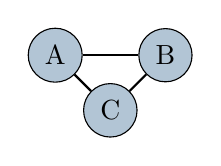
\begin{tikzpicture}[scale=0.7]
                    \node[draw, circle, fill=uibblue!30] (A) at (0,1) {A};
                    \node[draw, circle, fill=uibblue!30] (B) at (2,1) {B};
                    \node[draw, circle, fill=uibblue!30] (C) at (1,0) {C};
                    \draw[thick] (A) -- (B);
                    \draw[thick] (A) -- (C);
                    \draw[thick] (B) -- (C);
                \end{tikzpicture}
            \end{center}
        \end{column}
        
        \begin{column}{0.48\textwidth}
            \textbf{\faArrowRight\ Rettet graf (digraf):}
            \begin{itemize}
                \item Kantene har retning
                \item $A \rightarrow B \neq B \rightarrow A$
                \item Eksempel: Twitter-følgere
            \end{itemize}
            
            \begin{center}
                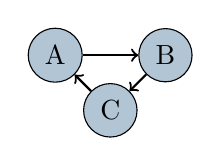
\begin{tikzpicture}[scale=0.7]
                    \node[draw, circle, fill=uibblue!30] (A) at (0,1) {A};
                    \node[draw, circle, fill=uibblue!30] (B) at (2,1) {B};
                    \node[draw, circle, fill=uibblue!30] (C) at (1,0) {C};
                    \draw[->, thick] (A) -- (B);
                    \draw[->, thick] (C) -- (A);
                    \draw[->, thick] (B) -- (C);
                \end{tikzpicture}
            \end{center}
        \end{column}
    \end{columns}
    
    \vspace{5mm}
    
    \begin{block}{Medisinsk kontekst}
        PSN (pasient-likhetsnettverk) er vanligvis \textbf{urettet}: likhet mellom A og B er symmetrisk.
    \end{block}
    
\end{frame}

% ---------------------------------------------------------------------
% N03
% ---------------------------------------------------------------------
\begin{frame}{N03: Vektet vs. uvektet graf}
    
    \begin{columns}
        \begin{column}{0.48\textwidth}
            \textbf{Uvektet graf:}
            \begin{itemize}
                \item Alle kanter er ``like''
                \item Binær: forbindelse eller ikke
            \end{itemize}
            
            \begin{center}
                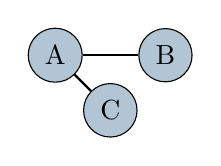
\begin{tikzpicture}[scale=0.7]
                    \node[draw, circle, fill=uibblue!30] (A) at (0,1) {A};
                    \node[draw, circle, fill=uibblue!30] (B) at (2,1) {B};
                    \node[draw, circle, fill=uibblue!30] (C) at (1,0) {C};
                    \draw[thick] (A) -- (B);
                    \draw[thick] (A) -- (C);
                \end{tikzpicture}
            \end{center}
        \end{column}
        
        \begin{column}{0.48\textwidth}
            \textbf{Vektet graf:}
            \begin{itemize}
                \item Kanter har numeriske vekter
                \item Representerer styrke/avstand
            \end{itemize}
            
            \begin{center}
                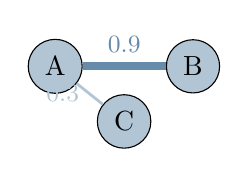
\begin{tikzpicture}[scale=0.7]
                    \node[draw, circle, fill=uibblue!30] (A) at (0,1) {A};
                    \node[draw, circle, fill=uibblue!30] (B) at (2.5,1) {B};
                    \node[draw, circle, fill=uibblue!30] (C) at (1.25,0) {C};
                    \draw[thick, line width=3pt, uibblue!60] (A) -- (B) node[midway, above] {\small 0.9};
                    \draw[thick, line width=1pt, uibblue!30] (A) -- (C) node[midway, left] {\small 0.3};
                \end{tikzpicture}
            \end{center}
        \end{column}
    \end{columns}
    
    \vspace{5mm}
    
    \begin{block}{I PSN}
        Vekten representerer \textbf{likhet} mellom pasienter. \\
        Høyere vekt = mer like pasienter.
    \end{block}
    
\end{frame}

% ---------------------------------------------------------------------
% N04
% ---------------------------------------------------------------------
\begin{frame}{N04: Nabomatrise (adjacency matrix)}
    
    \begin{columns}
        \begin{column}{0.4\textwidth}
            \begin{center}
                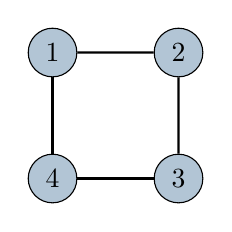
\begin{tikzpicture}[scale=0.8]
                    \node[draw, circle, fill=uibblue!30] (1) at (0,2) {1};
                    \node[draw, circle, fill=uibblue!30] (2) at (2,2) {2};
                    \node[draw, circle, fill=uibblue!30] (3) at (2,0) {3};
                    \node[draw, circle, fill=uibblue!30] (4) at (0,0) {4};
                    
                    \draw[thick] (1) -- (2);
                    \draw[thick] (1) -- (4);
                    \draw[thick] (2) -- (3);
                    \draw[thick] (3) -- (4);
                \end{tikzpicture}
            \end{center}
        \end{column}
        
        \begin{column}{0.55\textwidth}
            \textbf{Nabomatrise $A$:}
            
            \[
            A = \begin{pmatrix}
            0 & 1 & 0 & 1 \\
            1 & 0 & 1 & 0 \\
            0 & 1 & 0 & 1 \\
            1 & 0 & 1 & 0
            \end{pmatrix}
            \]
            
            \begin{itemize}
                \item $A_{ij} = 1$ hvis kant mellom $i$ og $j$
                \item $A_{ij} = 0$ ellers
                \item Symmetrisk for urettede grafer
            \end{itemize}
        \end{column}
    \end{columns}
    
    \vspace{5mm}
    
    \begin{block}{Vektet graf}
        I vektet graf: $A_{ij} = w_{ij}$ (vekten av kanten)
    \end{block}
    
\end{frame}

% =====================================================================
\section{Sentralitetsmål}
% =====================================================================

% ---------------------------------------------------------------------
% N05
% ---------------------------------------------------------------------
\begin{frame}{N05: Degree Centrality (grad-sentralitet)}
    
    \begin{columns}
        \begin{column}{0.5\textwidth}
            \begin{block}{Definisjon}
                \textbf{Degree} = antall kanter til en node
                \[
                C_D(v) = \frac{\deg(v)}{n-1}
                \]
                (normalisert: delt på maks mulige naboer)
            \end{block}
            
            \vspace{3mm}
            
            \textbf{Tolkning:}
            \begin{itemize}
                \item Høy degree = mange forbindelser
                \item ``Hub'' i nettverket
                \item Enkel å beregne
            \end{itemize}
        \end{column}
        
        \begin{column}{0.45\textwidth}
            \begin{center}
                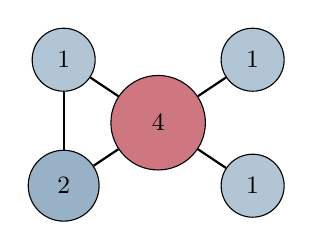
\begin{tikzpicture}[scale=0.8]
                    \node[draw, circle, fill=uibred!60, minimum size=1.2cm] (A) at (1.5,1.5) {\small 4};
                    \node[draw, circle, fill=uibblue!30, minimum size=0.8cm] (B) at (0,2.5) {\small 1};
                    \node[draw, circle, fill=uibblue!30, minimum size=0.8cm] (C) at (3,2.5) {\small 1};
                    \node[draw, circle, fill=uibblue!40, minimum size=0.9cm] (D) at (0,0.5) {\small 2};
                    \node[draw, circle, fill=uibblue!30, minimum size=0.8cm] (E) at (3,0.5) {\small 1};
                    
                    \draw[thick] (A) -- (B);
                    \draw[thick] (A) -- (C);
                    \draw[thick] (A) -- (D);
                    \draw[thick] (A) -- (E);
                    \draw[thick] (D) -- (B);
                \end{tikzpicture}
            \end{center}
            
            \textit{Node A har degree 4 (hub)}
        \end{column}
    \end{columns}
    
    \vspace{3mm}
    
    \begin{block}{Medisinsk relevans}
        I PSN: Pasienter med høy degree ligner på mange andre $\rightarrow$ ``typiske'' pasienter
    \end{block}
    
\end{frame}

% ---------------------------------------------------------------------
% N06
% ---------------------------------------------------------------------
\begin{frame}{N06: Betweenness Centrality (mellomliggenhet)}
    
    \begin{columns}
        \begin{column}{0.5\textwidth}
            \begin{block}{Definisjon}
                Andel korteste stier som går gjennom en node
                \[
                C_B(v) = \sum_{s \neq v \neq t} \frac{\sigma_{st}(v)}{\sigma_{st}}
                \]
                $\sigma_{st}$ = antall korteste stier fra $s$ til $t$
            \end{block}
            
            \vspace{3mm}
            
            \textbf{Tolkning:}
            \begin{itemize}
                \item Høy betweenness = ``bro'' mellom grupper
                \item Kontrollerer informasjonsflyt
                \item Kritisk for nettverkets struktur
            \end{itemize}
        \end{column}
        
        \begin{column}{0.45\textwidth}
            \begin{center}
                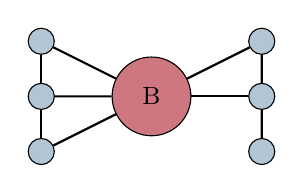
\begin{tikzpicture}[scale=0.7]
                    % Left cluster
                    \node[draw, circle, fill=uibblue!30] (A) at (0,2) {};
                    \node[draw, circle, fill=uibblue!30] (B) at (0,1) {};
                    \node[draw, circle, fill=uibblue!30] (C) at (0,0) {};
                    
                    % Bridge
                    \node[draw, circle, fill=uibred!60, minimum size=1cm] (X) at (2,1) {\small B};
                    
                    % Right cluster
                    \node[draw, circle, fill=uibblue!30] (D) at (4,2) {};
                    \node[draw, circle, fill=uibblue!30] (E) at (4,1) {};
                    \node[draw, circle, fill=uibblue!30] (F) at (4,0) {};
                    
                    \draw[thick] (A) -- (B) -- (C);
                    \draw[thick] (A) -- (X) -- (B);
                    \draw[thick] (C) -- (X);
                    \draw[thick] (X) -- (D);
                    \draw[thick] (X) -- (E);
                    \draw[thick] (D) -- (E) -- (F);
                \end{tikzpicture}
            \end{center}
            
            \textit{Node B er bro mellom to clusters}
        \end{column}
    \end{columns}
    
\end{frame}

% ---------------------------------------------------------------------
% N07
% ---------------------------------------------------------------------
\begin{frame}{N07: Eigenvector Centrality}
    
    \begin{block}{Idé}
        En node er viktig hvis den er koblet til \textbf{andre viktige noder}
    \end{block}
    
    \vspace{3mm}
    
    \begin{columns}
        \begin{column}{0.55\textwidth}
            \textbf{Beregning:}
            \[
            x_i = \frac{1}{\lambda} \sum_{j \in N(i)} x_j
            \]
            
            Eller i matriseform: $\mathbf{Ax} = \lambda \mathbf{x}$
            
            \vspace{3mm}
            
            \textbf{Forskjell fra degree:}
            \begin{itemize}
                \item Degree: teller bare antall naboer
                \item Eigenvector: vekter naboer etter deres viktighet
            \end{itemize}
        \end{column}
        
        \begin{column}{0.4\textwidth}
            \begin{center}
                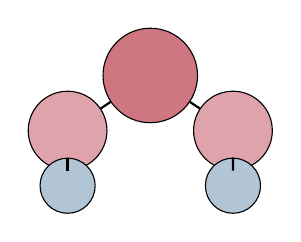
\begin{tikzpicture}[scale=0.7]
                    \node[draw, circle, fill=uibred!60, minimum size=1.2cm] (A) at (1.5,2) {};
                    \node[draw, circle, fill=uibred!40, minimum size=1cm] (B) at (0,1) {};
                    \node[draw, circle, fill=uibred!40, minimum size=1cm] (C) at (3,1) {};
                    \node[draw, circle, fill=uibblue!30, minimum size=0.7cm] (D) at (0,0) {};
                    \node[draw, circle, fill=uibblue!30, minimum size=0.7cm] (E) at (3,0) {};
                    
                    \draw[thick] (A) -- (B);
                    \draw[thick] (A) -- (C);
                    \draw[thick] (B) -- (D);
                    \draw[thick] (C) -- (E);
                \end{tikzpicture}
            \end{center}
            
            \textit{A har høyest eigenvector centrality}
        \end{column}
    \end{columns}
    
    \vspace{3mm}
    
    \begin{block}{Kjent anvendelse}
        Google PageRank er en variant av eigenvector centrality!
    \end{block}
    
\end{frame}

% ---------------------------------------------------------------------
% N08
% ---------------------------------------------------------------------
\begin{frame}{N08: Clustering Coefficient (klyngekoeffisient)}
    
    \begin{block}{Definisjon}
        Hvor mye naboene til en node er koblet til hverandre
        \[
        C_i = \frac{\text{antall kanter mellom naboer}}{\text{maks mulige kanter mellom naboer}}
        \]
    \end{block}
    
    \vspace{3mm}
    
    \begin{columns}
        \begin{column}{0.48\textwidth}
            \textbf{Høy clustering ($C = 1$):}
            \begin{center}
                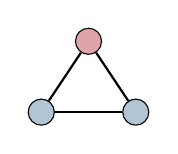
\begin{tikzpicture}[scale=0.6]
                    \node[draw, circle, fill=uibred!40] (A) at (1,2) {};
                    \node[draw, circle, fill=uibblue!30] (B) at (0,0.5) {};
                    \node[draw, circle, fill=uibblue!30] (C) at (2,0.5) {};
                    \draw[thick] (A) -- (B);
                    \draw[thick] (A) -- (C);
                    \draw[thick] (B) -- (C);
                \end{tikzpicture}
            \end{center}
            ``Naboene kjenner hverandre''
        \end{column}
        
        \begin{column}{0.48\textwidth}
            \textbf{Lav clustering ($C = 0$):}
            \begin{center}
                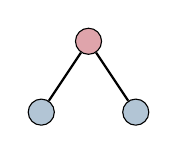
\begin{tikzpicture}[scale=0.6]
                    \node[draw, circle, fill=uibred!40] (A) at (1,2) {};
                    \node[draw, circle, fill=uibblue!30] (B) at (0,0.5) {};
                    \node[draw, circle, fill=uibblue!30] (C) at (2,0.5) {};
                    \draw[thick] (A) -- (B);
                    \draw[thick] (A) -- (C);
                    % No edge between B and C
                \end{tikzpicture}
            \end{center}
            ``Naboene kjenner ikke hverandre''
        \end{column}
    \end{columns}
    
    \vspace{3mm}
    
    \begin{block}{Medisinsk relevans}
        Høy clustering i PSN kan indikere tette pasientsubgrupper
    \end{block}
    
\end{frame}

% =====================================================================
\section{Community detection}
% =====================================================================

% ---------------------------------------------------------------------
% N09
% ---------------------------------------------------------------------
\begin{frame}{N09: Community Detection og Louvain-algoritmen}
    
    \begin{block}{Community Detection}
        Identifisere \textbf{grupper} (communities) av tett koblede noder
    \end{block}
    
    \vspace{3mm}
    
    \begin{columns}
        \begin{column}{0.5\textwidth}
            \textbf{Louvain-algoritmen:}
            \begin{enumerate}
                \item Start: hver node = egen gruppe
                \item Flytt noder til nabogrupper som øker \textbf{modularitet}
                \item Gjenta til ingen forbedring
                \item Aggreger og repeter hierarkisk
            \end{enumerate}
            
            \vspace{3mm}
            
            \textbf{Modularitet $Q$:}
            \begin{itemize}
                \item Måler kvalitet på inndeling
                \item $Q > 0.3$: god struktur
            \end{itemize}
        \end{column}
        
        \begin{column}{0.45\textwidth}
            \begin{center}
                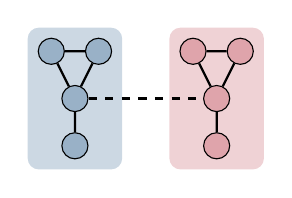
\begin{tikzpicture}[scale=0.6]
                    % Community 1
                    \fill[uibblue!20, rounded corners] (-0.5,-0.5) rectangle (1.5,2.5);
                    \node[draw, circle, fill=uibblue!40] (A) at (0,2) {};
                    \node[draw, circle, fill=uibblue!40] (B) at (1,2) {};
                    \node[draw, circle, fill=uibblue!40] (C) at (0.5,1) {};
                    \node[draw, circle, fill=uibblue!40] (D) at (0.5,0) {};
                    
                    % Community 2
                    \fill[uibred!20, rounded corners] (2.5,-0.5) rectangle (4.5,2.5);
                    \node[draw, circle, fill=uibred!40] (E) at (3,2) {};
                    \node[draw, circle, fill=uibred!40] (F) at (4,2) {};
                    \node[draw, circle, fill=uibred!40] (G) at (3.5,1) {};
                    \node[draw, circle, fill=uibred!40] (H) at (3.5,0) {};
                    
                    % Internal edges
                    \draw[thick] (A) -- (B) -- (C) -- (A);
                    \draw[thick] (C) -- (D);
                    \draw[thick] (E) -- (F) -- (G) -- (E);
                    \draw[thick] (G) -- (H);
                    
                    % Bridge edge
                    \draw[thick, dashed] (C) -- (G);
                \end{tikzpicture}
            \end{center}
            
            \textit{To identifiserte communities}
        \end{column}
    \end{columns}
    
\end{frame}

% ---------------------------------------------------------------------
% N10
% ---------------------------------------------------------------------
\begin{frame}{N10: NetworkX-biblioteket for Python}
    
    \begin{block}{NetworkX}
        Python-bibliotek for å opprette, manipulere og analysere grafer
    \end{block}
    
    \vspace{3mm}
    
    \textbf{Vanlige operasjoner:}
    
    \begin{columns}
        \begin{column}{0.48\textwidth}
            \texttt{\small import networkx as nx} \\[2mm]
            \texttt{\small \# Opprett graf} \\
            \texttt{\small G = nx.Graph()} \\
            \texttt{\small G.add\_edge('A', 'B', weight=0.8)} \\
            \texttt{\small G.add\_edge('B', 'C', weight=0.5)} \\[2mm]
            \texttt{\small \# Sentralitet} \\
            \texttt{\small nx.degree\_centrality(G)} \\
            \texttt{\small nx.betweenness\_centrality(G)}
        \end{column}
        
        \begin{column}{0.48\textwidth}
            \texttt{\small \# Community detection} \\
            \texttt{\small from community import louvain} \\
            \texttt{\small partition = louvain.best\_partition(G)} \\[2mm]
            \texttt{\small \# Visualisering} \\
            \texttt{\small nx.draw(G, with\_labels=True)} \\[2mm]
            \texttt{\small \# Fra nabomatrise} \\
            \texttt{\small G = nx.from\_numpy\_array(A)}
        \end{column}
    \end{columns}
    
    \vspace{5mm}
    
    \begin{block}{Ressurser}
        Dokumentasjon: \url{https://networkx.org/documentation/}
    \end{block}
    
\end{frame}

% ---------------------------------------------------------------------
% Oppsummering
% ---------------------------------------------------------------------
\begin{frame}{Oppsummering: N01--N10}
    
    \begin{columns}
        \begin{column}{0.48\textwidth}
            \textbf{Grafteori-grunnlag:}
            \begin{itemize}
                \item Graf = noder + kanter
                \item Rettet vs. urettet
                \item Vektet vs. uvektet
                \item Nabomatrise-representasjon
            \end{itemize}
            
            \vspace{3mm}
            
            \textbf{Sentralitetsmål:}
            \begin{itemize}
                \item Degree: antall forbindelser
                \item Betweenness: bro-rolle
                \item Eigenvector: viktige naboer
            \end{itemize}
        \end{column}
        
        \begin{column}{0.48\textwidth}
            \textbf{Strukturanalyse:}
            \begin{itemize}
                \item Clustering coefficient: lokal tetthet
                \item Community detection: finne grupper
                \item Louvain-algoritme: effektiv metode
            \end{itemize}
            
            \vspace{3mm}
            
            \textbf{Verktøy:}
            \begin{itemize}
                \item NetworkX (Python)
                \item Integrasjon med numpy/pandas
            \end{itemize}
        \end{column}
    \end{columns}
    
    \vspace{5mm}
    
    \begin{block}{Neste steg}
        Bruk disse konseptene til å bygge \textbf{pasient-likhetsnettverk} (PSN)!
    \end{block}
    
\end{frame}

\end{document}
